%%%%%%%%%%%%%%%%%%%%%%%%%%%%%%%%%%%%%%%%%%%%%%%%%%%%%%%%%%%%%%%%%%%%%%%%%%%%%%%%
% This chapter describes the analytics tools and views
%
% - Should rewrite comparison section, see pacivicVIS paper
%%%%%%%%%%%%%%%%%%%%%%%%%%%%%%%%%%%%%%%%%%%%%%%%%%%%%%%%%%%%%%%%%%%%%%%%%%%%%%%
\chapter{Enabling Analysis}
A comprehensive analytic system requires a variety of ways to manipulate and
looking at data. In this section we describe our solutions for trend detection,
making comparisons and high level overview.

% TODO: Maybe illustrate with an example
\section{Heatmap Perspective}
The heatmap�s data, in essence, is a time series data. There are multiple ways
we can view this time series to derive interesting patterns and trends. For this 
prototype we want to concentrate on comparability across different components
and time. For example, we want to ask: which vehicle component had more
complaints? which month had more complaints out of the year? 
To do this, we need to have multiple perspectives where data can be viewed from
different functional needs. We have provided the following perspectives in our
prototype:
\begin{itemize} [noitemsep]
  \item Month-Max: A monthly perspective where the importance score of each
  month is divided by the maximum monthly importance score over all components
  in the selected time.
  \item Component-Max: An object component perspective where the importance
  score of each month is divided by the maximum component score over the selected time.
  \item Global-Max: A global perspective where the month score is divided by the
  maximum score of all components over the selected time. 
\end{itemize}

We illustrate how the perspective scoring works with an example of a time over a
period of three month in table \ref{table:perspective}.
 
 
    % === Table ===
    \begin{table}[h]
	\begin{tabular}{| l | lll | lll | lll | lll | } 
	   % Column Heading
	   \hline
	   & \multicolumn{3}{|c|}{Score} & \multicolumn{3}{|c|}{Month} &
	   \multicolumn{3}{|c|}{Component} & \multicolumn{3}{|c|}{Global} \\
	   
	   % Data 
	   \hline
	   Engine & 1 & 10 & 100 &       % Original
	            10 & 15 & 100 &      % Month
	            100 & 100 & 100 &    % Component
	            100 & 100 & 100 \\   % Global
	            
	   Brake &  10 & 15 & 20  &      % Original
	            10 & 15 & 100 &      % Month
	            20 & 20 & 30  &      % Component
	            100 & 100 & 100 \\   % Global
	   \hline
	\end{tabular} \caption{Sample perspective
	based scores} \label{table:perspective}
	\end{table}
	% ============
  

Each of the perspectives above answers different questions and has its own
advantages and disadvantages. The month-max perspective allows us to compare 
component-to-component by month, but comparison against adjacent cells are 
meaningless because each cell uses a different base value. The component-max 
perspective is the opposite, it allows us to see trends with a single entity, 
but it does not allow comparison across components. Lastly, the global-max 
perspective is good at showing the outliers and supports both month-to-month 
and component-to-component comparisons, but it is difficult to see overall
trends because the outliers, if any, will dominate and push all non-outliers
into the same scoring bin.

To put the different perspectives in better context, we list sample 
questions that can be answered with these different perspective views:
\begin{itemize} [noitemsep]
  \item Month-Max: In month X, which vehicle component had the most complaints?
  \item Component-Max: Are there more braking problems in the summer months or
  the winter month?
  \item Global-Max: What are the most unreliable vehicle components?
\end{itemize}

The heatmap viewing perspective is at a global scope, thus a change in
perspective will affect all visible heatmaps. This keeps the interface
consistent and avoid viewers from switching to different modalities when they
shift their attention from one heatmap to another. The view switching mechanism
is realized as a drop-down control sitting atop the hierarchy filters and shows
the currently selected viewing mode.


    % === Figure === 
	\begin{figure}
	 \centering  
	 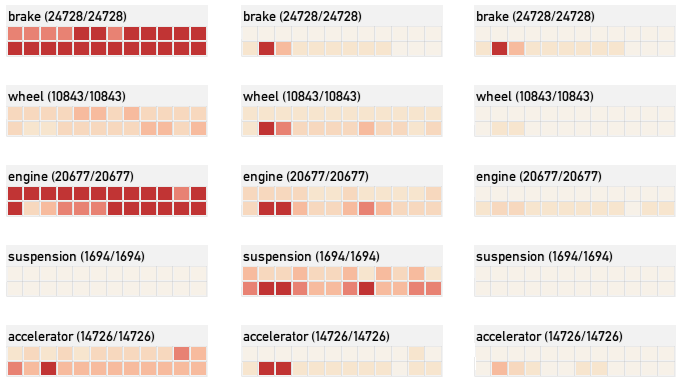
\includegraphics[width=\columnwidth]{heatmap.png}
	 \caption[Heatmap Perspectives]{Showing the different heatmap perspectives. Left
	 displays the monthly perspective, centre displays the component perspective, and right displays the
	 global perspective}
	 \label{figure:heatmap}
	\end{figure}
	% ==============

\section{Comparison}
Comparison mode allows people to compare two different types of the same
physical product specified by two different query sets Q1 and Q2. Every entity
from a query set is matched against the same named entity in the other query
set, producing an entity level based comparison. For example, we can compare how
each car component fared against each other in a comparison of Honda Civic
versus Toyota Corolla, or comparing Ford Focus against the industry form.

Two separate measures are used for the comparison view. A contribution sum and a
percentage difference. The contribution sum is the aggregated entity score from
the two query sets, it reflects the overall importance of the entity by
emphasizing the frequently occurring entities in one or both query set. The
percentage difference describes the relative frequencies of an entity, whether
it occurs more frequently under Q1 or Q2 relative to the total contributions
from Q1 and Q2 respectively. The percentage score is calculated as entity score
divided by the total contribution. Then the percentage difference follows as
percentage score Q1 minus percentage score Q2, with the sign and magnitude
indicating  which query set has the stronger presence. We made the decision to
use percentage based comparisons because it enables as to compare query results
of different sizes.

%%%%%%%%%%%%%%%%%%%%%%%%%%%%%%%%%%%%%%%%%%%%%%%%%%%%%%%%%%%%%%%%%%%%%%%%%%%%%%%%
\section{Viewing Modes}
A comprehensive analytic system requires a variety of ways to manipulate and
looking at data. In this section we describe our solutions for trend detection,
making comparisons and high level overview.

% TODO: Maybe illustrate with an example
\subsection{Heatmap Perspective}
The heatmap�s data, in essence, is a time series data. There are multiple ways
we can view this time series to derive interesting patterns and trends. For this 
prototype we want to concentrate on comparability across different components
and time. For example, we want to ask: which vehicle component had more
complaints? which month had more complaints out of the year? 
To do this, we need to have multiple perspectives where data can be viewed from
different functional needs. We have provided the following perspectives in our
prototype:
\begin{itemize} [noitemsep]
  \item Month-Max: A monthly perspective where the importance score of each
  month is divided by the maximum monthly importance score over all components
  in the selected time.
  \item Component-Max: An object component perspective where the importance
  score of each month is divided by the maximum component score over the selected time.
  \item Global-Max: A global perspective where the month score is divided by the
  maximum score of all components over the selected time. 
\end{itemize}

We illustrate how the perspective scoring works with an example of a time over a
period of three month in table \ref{table:perspective}.
 
 
    % === Table ===
    \begin{table}[h]
	\begin{tabular}{| l | lll | lll | lll | lll | } 
	   % Column Heading
	   \hline
	   & \multicolumn{3}{|c|}{Score} & \multicolumn{3}{|c|}{Month} &
	   \multicolumn{3}{|c|}{Component} & \multicolumn{3}{|c|}{Global} \\
	   
	   % Data 
	   \hline
	   Engine & 1 & 10 & 100 &       % Original
	            10 & 15 & 100 &      % Month
	            100 & 100 & 100 &    % Component
	            100 & 100 & 100 \\   % Global
	            
	   Brake &  10 & 15 & 20  &      % Original
	            10 & 15 & 100 &      % Month
	            20 & 20 & 30  &      % Component
	            100 & 100 & 100 \\   % Global
	   \hline
	\end{tabular} \caption{Sample perspective
	based scores} \label{table:perspective}
	\end{table}
	% ============
  

Each of the perspectives above answers different questions and has its own
advantages and disadvantages. The month-max perspective allows us to compare 
component-to-component by month, but comparison against adjacent cells are 
meaningless because each cell uses a different base value. The component-max 
perspective is the opposite, it allows us to see trends with a single entity, 
but it does not allow comparison across components. Lastly, the global-max 
perspective is good at showing the outliers and supports both month-to-month 
and component-to-component comparisons, but it is difficult to see overall
trends because the outliers, if any, will dominate and push all non-outliers
into the same scoring bin.

To put the different perspectives in better context, we list sample 
questions that can be answered with these different perspective views:
\begin{itemize} [noitemsep]
  \item Month-Max: In month X, which vehicle component had the most complaints?
  \item Component-Max: Are there more braking problems in the summer months or
  the winter month?
  \item Global-Max: What are the most unreliable vehicle components?
\end{itemize}

The heatmap viewing perspective is at a global scope, thus a change in
perspective will affect all visible heatmaps. This keeps the interface
consistent and avoid viewers from switching to different modalities when they
shift their attention from one heatmap to another. The view switching mechanism
is realized as a drop-down control sitting atop the hierarchy filters and shows
the currently selected viewing mode.


    % === Figure === 
	\begin{figure}
	 \centering  
	 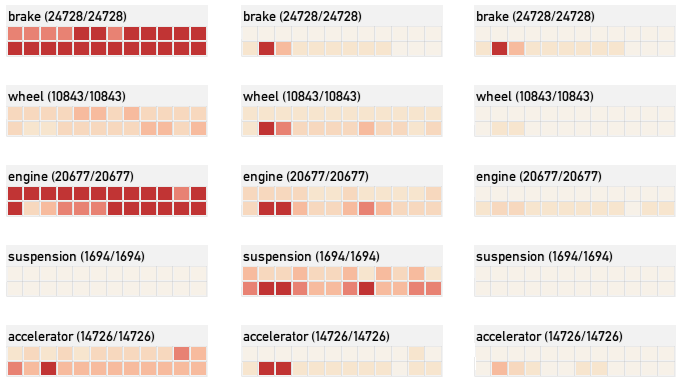
\includegraphics[width=\columnwidth]{heatmap.png}
	 \caption[Heatmap Perspectives]{Showing the different heatmap perspectives. Left
	 displays the monthly perspective, centre displays the component perspective, and right displays the
	 global perspective}
	 \label{figure:heatmap}
	\end{figure}
	% ==============

\subsection{Comparison}
Comparison mode allows people to compare two different types of the same
physical product specified by two different query sets Q1 and Q2. Every entity
from a query set is matched against the same named entity in the other query
set, producing an entity level based comparison. For example, we can compare how
each car component fared against each other in a comparison of Honda Civic
versus Toyota Corolla, or comparing Ford Focus against the industry form.

Two separate measures are used for the comparison view. A contribution sum and a
percentage difference. The contribution sum is the aggregated entity score from
the two query sets, it reflects the overall importance of the entity by
emphasizing the frequently occurring entities in one or both query set. The
percentage difference describes the relative frequencies of an entity, whether
it occurs more frequently under Q1 or Q2 relative to the total contributions
from Q1 and Q2 respectively. The percentage score is calculated as entity score
divided by the total contribution. Then the percentage difference follows as
percentage score Q1 minus percentage score Q2, with the sign and magnitude
indicating  which query set has the stronger presence. We made the decision to
use percentage based comparisons because it enables as to compare query results
of different sizes.

We encode the sum score as the colour of the \threed component, based on the
default colour scale. For the difference score, we render the measure as an
outline around the object. The sign of the difference is encoded as one of two diverging
colours, one for positive and one for negative values. The magnitude of the
difference is encoded as the transparency of the outline, larger magnitude have
more distinct, solid outlines compared to smaller values. Thus, a highly
problematic object from both side will have a strong presence overall but with a
faint outline, while a lopsided but infrequent problem will have strong outline
but barely visible interior colour.

As an example, see Figure \ref{figure:comparison}, where we compared Plymouth
against both the Jeep and Chrysler. At a glance most parts remain the same
with the exception of two outliers, Jeep appear to have a higher failure rate
than Plymouth, and Dodge has a higher failure rate in brakes component. The
overview could suggest that Plymouth is more reliable than both vehicles.
 
    % === Figure ===
	\begin{figure}
	 \centering  
	 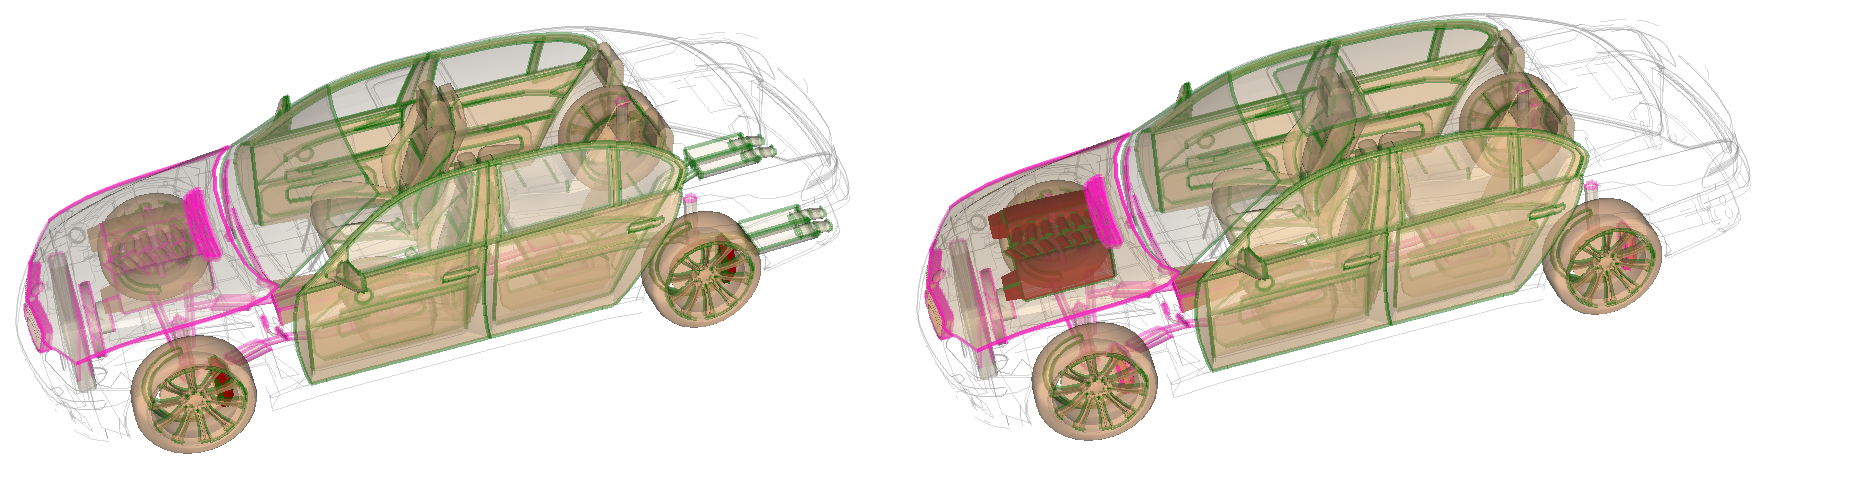
\includegraphics[width=\columnwidth]{comparison.png}
	 \caption[Comparison View]{Left: Plymouth versus Chrysler, the brake appears to
	 be the dominant issue and Make 14 has the higher rate of complaints. Right:
	 Plymouth versus Jeep, the engine is the dominant issue and Make 1 has higher
	 rate of complaints.}
	 \label{figure:comparison}
	\end{figure}
	% ==============
 
By default, comparison mode is turned off. It is activated when the viewer
switches the second hierarchy filter from the ``None'' position to a valid
selection. Subsequent query modifications are carried out in comparison mode
until the selection is turned to ``None'' again.

One limitation with this approach is our current usage of the total
contributions to calculate the percentage scores. Our total contribution is in
relations to the number of documents in the corpus, which may or may not be a
good indication of the overall contribution. 

 
 
\section{Aggregation}
By default, the system treats each object individually rather than object
groups. For example ``seatbelt'', ``backrest'' and ``seat'' are all scored
separately, even though they are logically under the group ``seat''. This
setting allows people to isolate and identify unique problems accurately. There
are times, however, when this level of information is unnecessarily detailed and
a higher level of abstraction is desirable.

    % === Figure === 
	\begin{figure}
	 \centering  
	 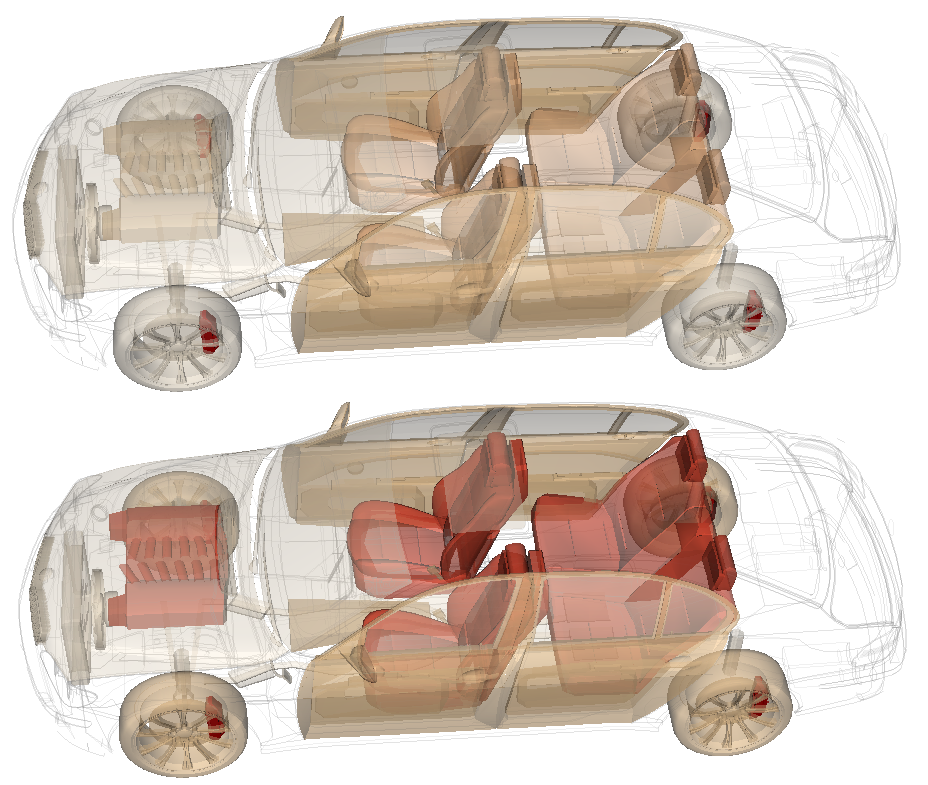
\includegraphics[width=\columnwidth]{aggregation.png}
	 \caption[Aggregation View]{Top: Aggregation mode disabled. Bottom: Aggregation
	 mode enabled, note that the seat and engine now appears more prominent in the visualization.}
	 \label{figure:aggregation}
	\end{figure}
	% ==============
	
Aggregation mode mimics the type of high level rating system found on consumers
review websites. When aggregation mode is enabled, individual objects, and their
scores are aggregated up to the first level entities. In our specific case, the 
first level are the major sub-systems in a vehicle. The visualization responds
by making all child objects referencing the aggregated score of their parent
subsystem. 

Aggregation mode is enabled/disabled by a toggle switch located at the top
portion of the interface. Aggregation mode works in
conjunction with comparison mode, allow people to make comparison of major systems.

An example is shown in Figure \ref{figure:aggregation}. A default rendering is
shown in the top portion, one can see that brake is the most severe out of all
components. The bottom shows the aggregated view, one can observe that on a
higher level, the engine and seat subsystems are quite problematic.
 
